A subdivision surface is the limit surface resulted from the
application of a subdivision algorithm to a control polyhedron
(Figure \ref{fig:teaser}). The subdivision algorithm  
recursively \emph{refine} (subdivide) the control polyhedron 
and \emph{modify} (smooth) the geometry. 
A subdivision algorithm can be characterized 
by its \emph{refinement operator} and 
\emph{modification operator(s)}. 

The refinement operator edits the connectivity
and create a uniformly refined mesh from the source polyhedron.
Refinement operators are classified according to the connectivity
pattern and the topology correspondence. 
Figure \ref{RefSchemes} shows four major refinements employed
in subdivision algorithms, which include 
Catmull-Clark subdivision (PQQ) \cite{cc},
Loop subdivision (PTQ) \cite{loop}, 
Doo-Sabin subdivision (DQQ) \cite{ds}
and $\sqrt{3}$ subdivision \cite{sqrt3}.
Subdivisions, such as Quad-Triangle subdivision (PQQ + PTQ) \cite{sqt},
may employ a hybrid refinement combining two reinements.

\begin{figure}
  \centering
  \psfrag{PQQ}[]{\scriptsize PQQ} 
  \psfrag{PTQ}[]{\scriptsize PTQ}
  \psfrag{DQQ}[]{\scriptsize DQQ} 
  \psfrag{Sqrt3}[]{\scriptsize $\sqrt{3}$} 
  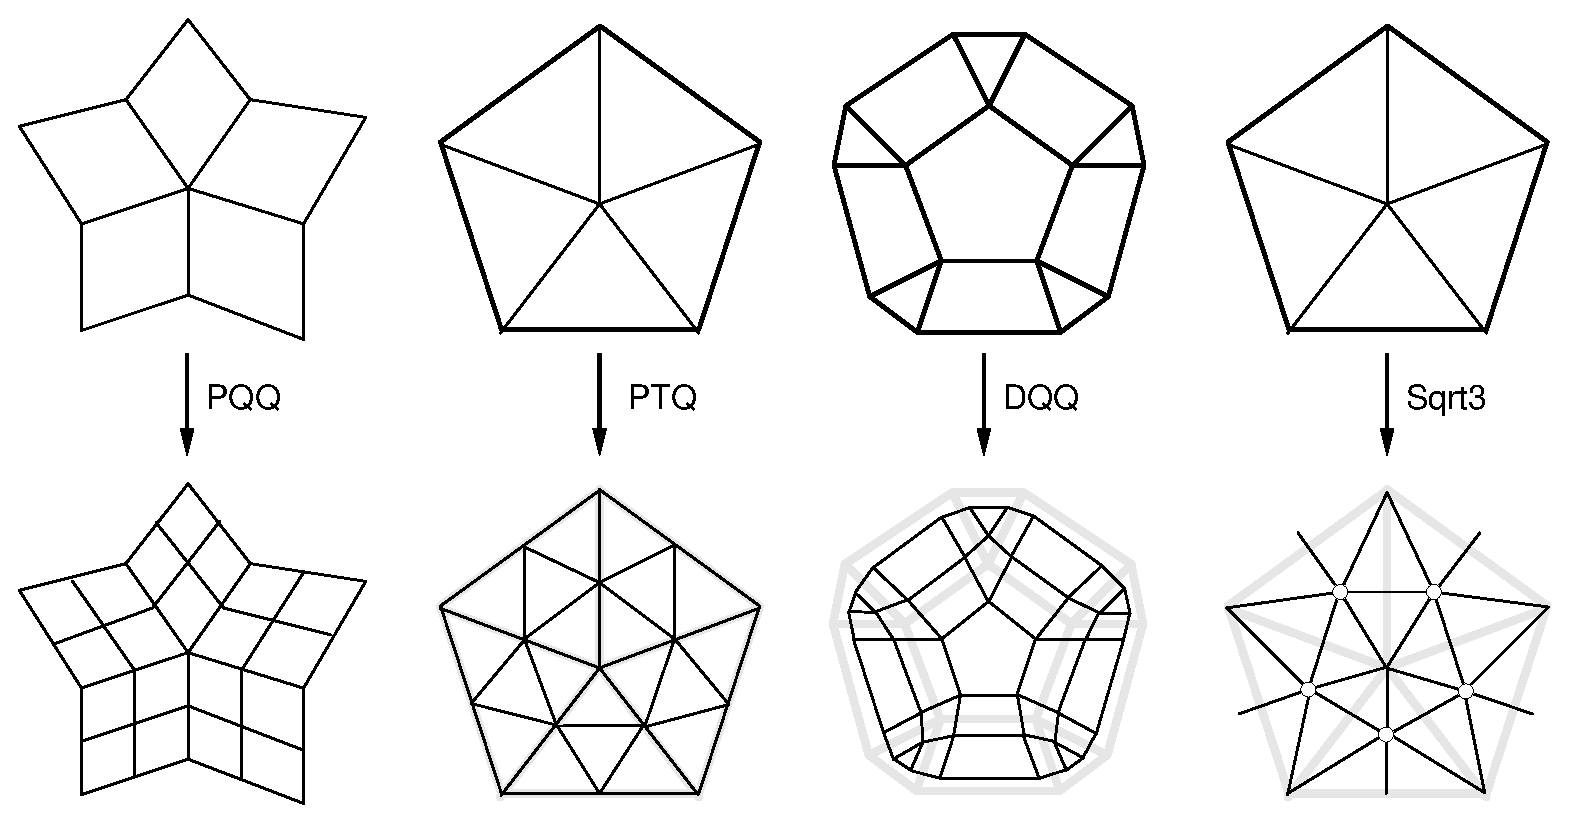
\epsfig{file=pfigs/RefSchemes.eps, width=4in}
  \caption{Refinement operators: 
    primal quadrilateral quadrisection (PQQ),
    primal triangle quadrisection (PTQ),
    dual quadrilateral quadrisection (DQQ) and
    $\sqrt{3}$ triangulation.}
  \label{fig:RefSchemes}
\end{figure}

The modification operator collects the stencil (submesh) of 
the source polyhedron and applied a mask (weighted map) 
on the submesh to generate the corresponding vertex of 
the target (refined) polyhedron. Figure \ref{fig:RefMap} 
demonstrates the examples of the correspondence 
between a stencil and its smoothed vertices. Subdivisions
usually have several modification operators with different
different types of stencils (Figure \ref{fig:RefMap} (a-c)). 

\begin{figure}
  \centering
  \psfrag{A}[]{(a)}
  \psfrag{B}[]{(b)}
  \psfrag{C}[]{(c)}
  \psfrag{D}[]{(d)}
  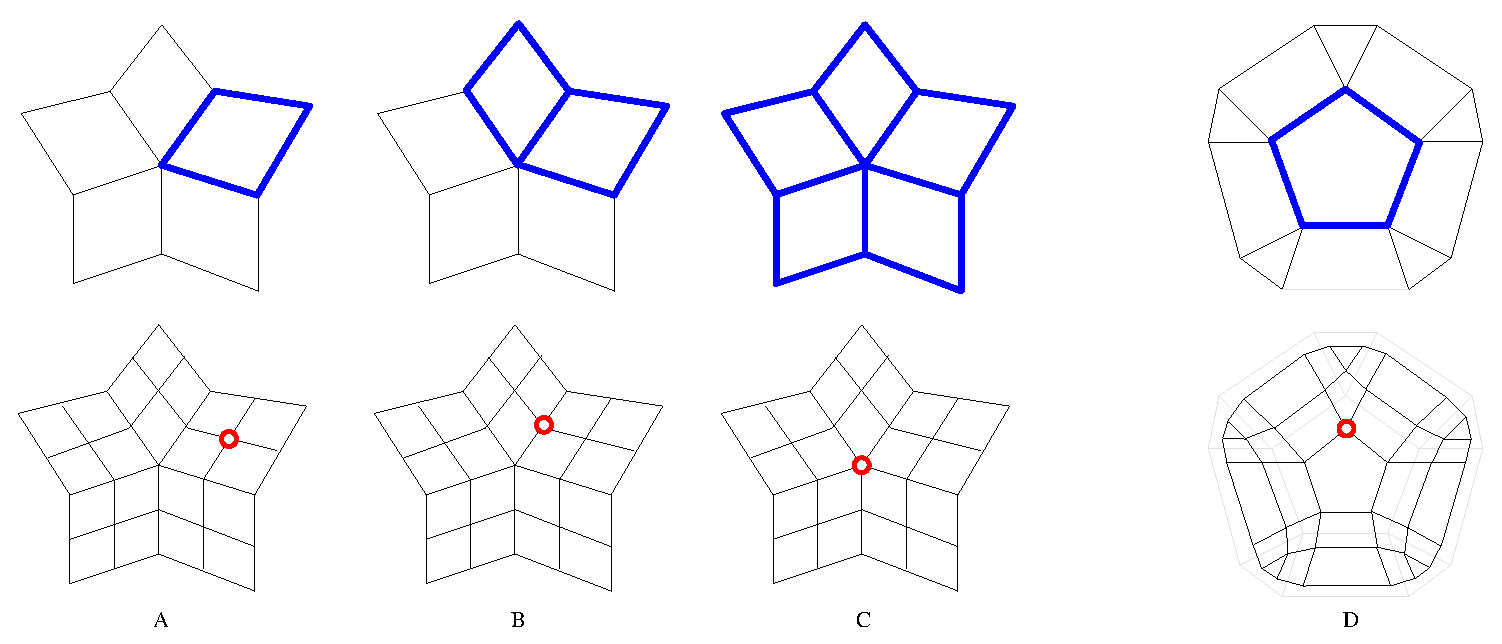
\epsfig{file=pfigs/RefMap.eps, width=4.5in}
  \caption{The correspondence of the stencil and the 
           target vertex in the Catmull-Clark subdivision (a-c)
	   and Doo-Sabin subdivision (d). Catmull-Clark
	   subdivsion has three stencils: facet-stencil (a), 
	   edge-stencil (b) and vertex-stencil (c).}
  \label{fig:RefMap}
\end{figure}

%% Any implementation of a subdivision scheme contains two major
%% components: \italic{refinement scheme} and \italic{geometry rules}.
%% Refinement schemes are defined by the 
%% \italic{uniform connectivity reconfiguration} of the source 
%% mesh (the domain) to the target mesh (the range). The geometry rules,
%% providing certain surface properties, e.g the smoothness, are the
%% mapping functions of the \italic{footprints} in the domain mesh to the
%% \italic{vertices} in the range mesh. Any subdivision in practice can
%% be defined as a legal combination of a refinement scheme and the
%% geometry rules. Based on the paradigm of the
%% \italic{policy-based design} \cite{a-rotm-02}, the combination can be
%% designed as the \italic{host function} (the refinement function)
%% templated with the \italic{policy class} (the geometry rules).

In this tutorial, the design of subdivisions focuses on how
to implement connectivity editing of the refinement operators
and how to locate the correspondences between the stencil and the
smoothed vertex.
  
A compelete introduction on subdisviions can be find at 
\cite{siggraph1998notes}.
